\documentclass[onecolumn,oneside,letterpaper,12pt]{article} 

\usepackage{geneticsSupT}
%\usepackage{geneticsT2}

\usepackage{times}
\usepackage{color}

% rayout %
\addtolength{\oddsidemargin}{-2.75cm}
\addtolength{\evensidemargin}{-0.75cm}

\addtolength{\textwidth}{5.5cm}
\addtolength{\topmargin}{-3cm}
\addtolength{\textheight}{4.5cm}

\parindent=1em
\setlength{\parskip}{0.01pt}

\renewcommand{\textfraction}{0.01}
\renewcommand{\topfraction}{0.99}
\renewcommand{\bottomfraction}{0.65}
\renewcommand{\floatpagefraction}{0.90}
\renewcommand{\dbltopfraction}{0.95}
\renewcommand{\dblfloatpagefraction}{0.80}
\renewcommand{\sfdefault}{phv}

\usepackage{fancyhdr}
\pagestyle{fancy}
\fancyhf{}
\fancyfoot[CE,CO]{\thepage}
\renewcommand{\headrulewidth}{0pt}
\fancypagestyle{plain}{
	\fancyhf{}
}

% space of double hline in Table
\doublerulesep = 0.4pt

\title{The molecular basis of parallel adaptation to\\ highland climate in domesticated maize.}

\author{
 Shohei Takuno, Peter Ralph, Sofiane Mezmouk, Kelly Swarts, Matthew B. Hufford, Rob J. Elshire, Jeffrey C. Glaubitz, Edward S. Buckler and Jeffrey Ross-Ibarra
   }

\usepackage{natbib}
\bibpunct{(}{)}{;}{a}{}{,}

\usepackage{amsmath}

\usepackage{graphicx}

\begin{document}

\maketitle

% Supplemental 

Later we should separate all Text S1, figs and tables in this file if we submit PLoS G.

\newpage

\renewcommand{\thefigure}{\Roman{figure}} 
% Figure AllelePat is not called in the main text, and I use Roman numbers for figure numbers

\noindent {\Large \textit{Text~S1} }

We classified the patterns of allelic differentiation among highland and lowland populations in Mexico and S. America together with the information of \emph{parviglumis} in an \emph{ad hoc} manner; the allelic differentiation pattern is consistent with highland or lowland adaptation scenario.  
In Figure~\ref{AllelePat}, we illustrate the frequency of putative ancestral and derived alleles in the five populations, drawn by red and blue, respectively.

First, we focus on the SNPs with the signature of adaptation only in Mexican populations (Figure~\ref{AllelePat}A).  
The first and second rows shows the typical patterns of highland adaptation with \emph{parviglumis} data available.
We simply assume that the allele in higher frequency in \emph{parviglumis} is ancestral.
Both rows show the consistent pattern to highland adaptation in Mexico because the frequency of the putative derived allele in Mexican highlands is highly differentiated from those in both \emph{parviglumis} and Mexican lowlands.
The patterns in S. America are different between the first and second rows.
However, we do not take the patterns in S. American populations into account because there is no adaptive signature in S. American.
On the other hand, we should consider the allelic pattern in S. America in the case of the third row; we cannot utilize the information of \emph{parviglumis}.
It is impossible to infer the ancestral allele, so we assume the pattern is consistent with highland adaptation if one allele is in higher frequency in Mexican lowlands and S. American populations and the others is in higher frequency in Mexican highlands.
We classified the SNPs into lowland adaptation in the same way (from fourth to sixth rows in Figure~\ref{AllelePat}A).

Next, we consider the SNPs with the signatures of adaptation in both Mexico and S. America (Figure~\ref{AllelePat}B).
The pattern in the first row is consistent with parallel highland adaptation, whereas the second row shows parallel lowland adaptation. 
We cannot infer lowland or highland adaptation without the outgroup, so we ignore such SNPs.
The pattern in the third row is the special case: the allele frequency is similar between Mexican lowlands and S. American highlands and similar between Mexican highlands and S. American lowlands.
This pattern could be explained by that the SNP is linked to a read adaptive SNP and recombination breaks down the linkage between them.

Finally, we tested whether PHS test supports highland and lowland adaptation scenario.
Consider the case of highland adaptation.
We assumed that the putative derived allele is adaptive in highlands and checked whether the haplotype length is longer in highlands than that in lowlands.
However, haplotype length cannot be compared directly because the derived allele frequency is different between highlands and lowlands.
Thus, we compared the \emph{P}-values of PHS test as a indicator of haplotype length given allele frequency (Pr($PHS_{xA}\leq PHS_{null|p}$ in Materials and Methods).
We just say that the PHS test is consistent if the \emph{P}-value in highlands is smaller than the \emph{P}-value in lowlands (haplotype length is longer as \emph{P}-value is smaller).
The result is summarized in Table~S3.



%%%%%%%%%%%%%%%%%%%%%%%%%%%%%%%%%%%%%%%%%%%%%%%%%%%%%%%%%%%%
\begin{figure}[b]
  \begin{center}
    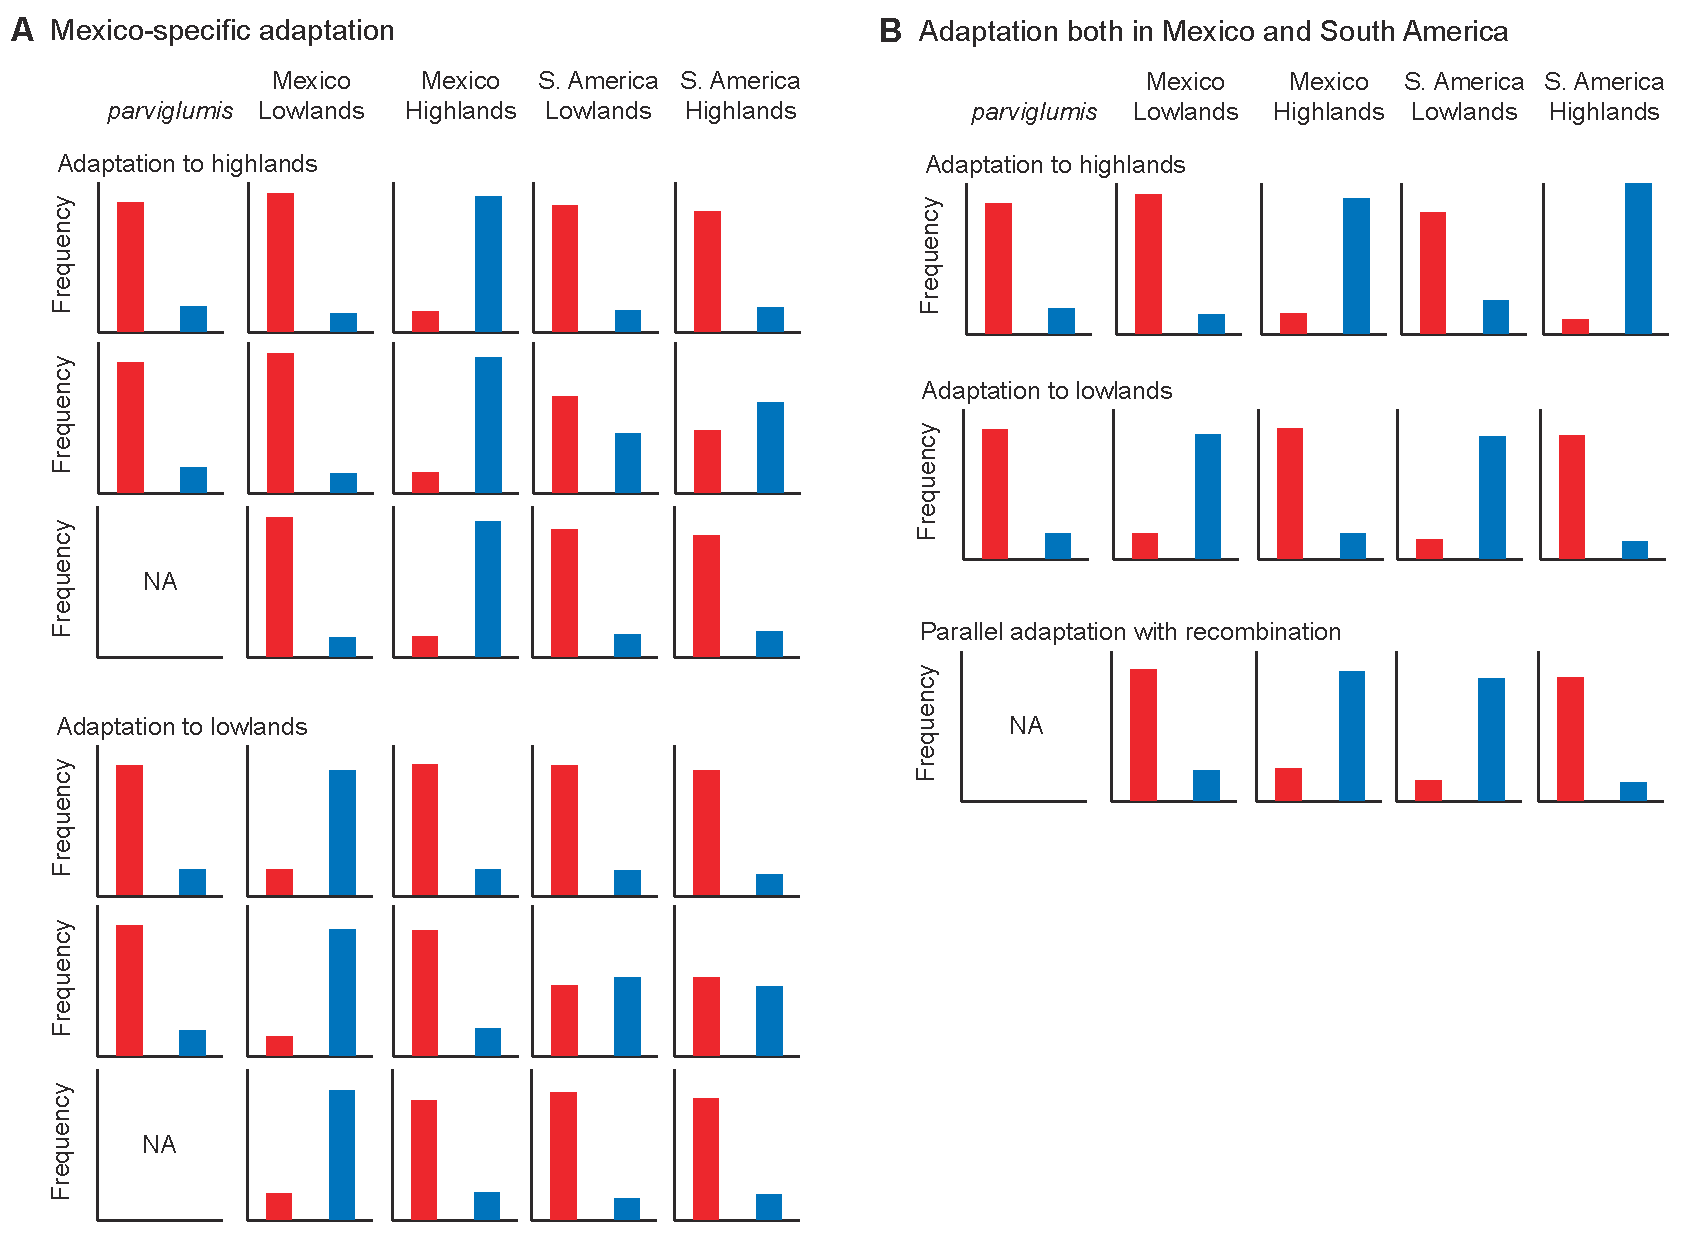
\includegraphics[width=0.9\columnwidth]{fig/AllelePat.pdf}
    \caption{Illustration of allele frequency changes in maize and \emph{parviglumis}.  Red and blue bars represent the allele frequency of ancestral and derived, adaptive alleles, respectively.  The allele frequencies in the five populations are shown: \emph{parviglumis}, Mexican lowlands and highlands, and S. America lowlands and highlands. NA in \emph{parviglumis} indicates that there is no SNP data in the site.}
    \label{AllelePat}
  \end{center}
\end{figure}
%%%%%%%%%%%%%%%%%%%%%%%%%%%%%%%%%%%%%%%%%%%%%%%%%%%%%%%%%%%%

\clearpage
\suppl

%\section*{SUPPLEMENTAL METHODS}



%%%%%%%%%%%%%%%%%%%%%%%%%%%%%%%
%Table S1 %
\renewcommand{\arraystretch}{1.2}

\begin{table}[h]
    \begin{center}
    \caption[]{List of maize landraces used in this study\hspace*{7.5cm}}  
{\fontsize{7}{10}\selectfont
%{\small
    \begin{tabular}{llllllllll}
        \hline\hline
       & & & \\[-4mm] 
	 ID$^a$	&	USDA ID	&	Population	&	Landrace	&	Locality	&	Latitude	&	Longitude	&	Elevation	&	Origin	\\[0.0cm]
	\hline 
	& & & \\[-4mm] 
{\bf RIMMA0409}	&	PI 478968	&	Mexico 	&	Tepecintle	&	Chiapas, Mexico	&	15.4 	&	-92.9 	&	107	&	USDA	\\
RIMMA0410	&	PI 478970	&	Lowland	&	Vandeno	&	Chiapas, Mexico	&	15.4 	&	-92.9 	&	107	&	USDA	\\
{\bf RIMMA0433}	&	PI 490825	&		&	Nal Tel ATB	&	Chiquimula, Guatemala	&	14.7 	&	-89.5 	&	457	&	USDA	\\
{\bf RIMMA0441}	&	PI 515538	&		&	Coscomatepec	&	Veracruz, Mexico	&	19.2 	&	-97.0 	&	1320	&	USDA	\\
{\bf RIMMA0615}	&	PI 628480	&		&	Tuxpeno	&	Puebla, Mexico	&	20.1 	&	-97.2 	&	152	&	USDA	\\
{\bf RIMMA0619}	&	PI 645772	&		&	Pepitilla	&	Guerrero, Mexico	&	18.4 	&	-99.5 	&	747	&	USDA	\\
{\bf RIMMA0628}	&	PI 646017	&		&	Tuxpeno Norteno	&	Tamaulipas, Mexico	&	23.3 	&	-99.0 	&	300	&	USDA	\\
{\bf RIMMA0696}	&	Ames 28568	&		&	Tuxpeno	&	El Progreso, Guatemala	&	16.5 	&	-90.2 	&	30	&	Goodman	\\
{\bf RIMMA0700}	&	NSL 291626	&		&	Olotillo	&	Chiapas, Mexico	&	16.8 	&	-93.2 	&	579	&	Goodman	\\
{\bf RIMMA0701}	&	PI 484808	&		&	Olotillo	&	Chiapas, Mexico	&	16.6 	&	-92.7 	&	686	&	Goodman	\\
{\bf RIMMA0702}	&	Ames 28534	&		&	Negro de Tierra Caliente	&	Sacatepequez, Guatemala	&	14.5 	&	-90.8 	&	1052	&	Goodman	\\
{\bf RIMMA0703}	&	NSL 283390	&		&	Nal Tel	&	Yucatan, Mexico	&	20.8 	&	-88.5 	&	30	&	Goodman	\\
{\bf RIMMA0709}	&	Ames 28452	&		&	Tehua	&	Chiapas, Mexico	&	16.5 	&	-92.5 	&	747	&	Goodman	\\
{\bf RIMMA0710}	&	PI 478988	&		&	Tepecintle	&	Chiapas, Mexico	&	15.3 	&	-92.6 	&	91	&	Goodman	\\
{\bf RIMMA0712}	&	NSL 291696 CYMT	&		&	Oloton	&	Baja Verapaz, Guatemala	&	15.3 	&	-90.3 	&	1220	&	Goodman	\\
{\bf RIMMA0716}	&	Ames 28459	&		&	Zapalote Grande	&	Chiapas, Mexico	&	15.3 	&	-92.7 	&	91	&	Goodman	\\
{\bf RIMMA0720}	&	PI 489372	&		&	Negro de Tierra Caliente	&	Guatemala	&	15.5 	&	-88.9 	&	39	&	Goodman	\\
{\bf RIMMA0721}	&	Ames 28485	&		&	Nal Tel ATB	&	Chiquimula, Guatemala	&	14.6 	&	-90.1 	&	915	&	Goodman	\\
{\bf RIMMA0722}	&	Ames 28564	&		&	Dzit Bacal	&	Jutiapa, Guatemala	&	14.3 	&	-89.7 	&	737	&	Goodman	\\
{\bf RIMMA0727}	&	Ames 28555	&		&	Comiteco	&	Guatemala	&	14.4 	&	-90.5 	&	1151	&	Goodman	\\
{\bf RIMMA0729}	&	PI 504090	&		&	Tepecintle	&	Guatemala	&	15.4 	&	-89.7 	&	122	&	Goodman	\\
{\bf RIMMA0730}	&	Ames 28517	&		&	Quicheno Late	&	Sacatepequez, Guatemala	&	14.5 	&	-90.8 	&	1067	&	Goodman	\\
{\bf RIMMA0731}	&	PI 484137	&		&	Bolita	&	Oaxaca, Mexico	&	16.8 	&	-96.7 	&	1520	&	Goodman	\\
{\bf RIMMA0733}	&	PI 479054	&		&	Zapalote Chico	&	Oaxaca, Mexico	&	16.6 	&	-94.6 	&	107	&	Goodman	\\
	\hline 
	& & & \\[-4mm] 
{\bf RIMMA0416}	&	PI 484428	&	Mexico	&	Cristalino de Chihuahua	&	Chihuahua, Mexico	&	29.4 	&	-107.8 	&	2140	&	NA	\\
{\bf RIMMA0417}	&	PI 484431	&	Highland	&	Azul	&	Chihuahua, Mexico	&	28.6 	&	-107.5 	&	2040	&	USDA	\\
{\bf RIMMA0418}	&	PI 484476	&		&	Gordo	&	Chihuahua, Mexico	&	28.6 	&	-107.5 	&	2040	&	USDA	\\
{\bf RIMMA0421}	&	PI 484595	&		&	Conico	&	Puebla, Mexico	&	19.9 	&	-98.0 	&	2250	&	USDA	\\
{\bf RIMMA0422}	&	PI 485071	&		&	Elotes Conicos	&	Puebla, Mexico	&	19.1 	&	-98.3 	&	2200	&	USDA	\\
{\bf RIMMA0423}	&	PI 485116	&		&	Cristalino de Chihuahua	&	Chihuahua, Mexico	&	29.2 	&	-108.1 	&	2095	&	NA	\\
{\bf RIMMA0424}	&	PI 485120	&		&	Apachito	&	Chihuahua, Mexico	&	28.0 	&	-107.6 	&	2400	&	USDA	\\
{\bf RIMMA0425}	&	PI 485128	&		&	Palomero Tipo Chihuahua	&	Chihuahua, Mexico	&	26.8 	&	-107.1 	&	2130	&	USDA	\\
{\bf RIMMA0614}	&	PI 628445	&		&	Mountain Yellow	&	Jalisco, Mexico	&	20.0 	&	-103.8 	&	2060	&	USDA	\\
{\bf RIMMA0616}	&	PI 629202	&		&	Zamorano Amarillo	&	Jalisco, Mexico	&	20.8 	&	-102.8 	&	1800	&	USDA	\\
{\bf RIMMA0620}	&	PI 645786	&		&	Celaya	&	Guanajuato, Mexico	&	20.2 	&	-100.9 	&	1799	&	USDA	\\
{\bf RIMMA0621}	&	PI 645804	&		&	Zamorano Amarillo	&	Guanajuato, Mexico	&	21.1 	&	-101.7 	&	1870	&	USDA	\\
{\bf RIMMA0623}	&	PI 645841	&		&	Palomero de Jalisco	&	Jalisco, Mexico	&	20.0 	&	-103.7 	&	2520	&	USDA	\\
{\bf RIMMA0625}	&	PI 645984	&		&	Cacahuacintle	&	Puebla, Mexico	&	19.0 	&	-97.4 	&	2600	&	USDA	\\
RIMMA0626	&	PI 645993	&		&	Arrocillo Amarillo	&	Puebla, Mexico	&	19.9 	&	-97.6 	&	2260	&	USDA	\\
{\bf RIMMA0630}	&	PI 646069	&		&	Arrocillo Amarillo	&	Veracruz, Mexico	&	19.8 	&	-97.3 	&	2220	&	USDA	\\
{\bf RIMMA0670}	&	Ames 28508	&		&	San Marceno	&	San Marcos, Guatemala	&	15.0 	&	-91.8 	&	2378	&	Goodman	\\
{\bf RIMMA0671}	&	Ames 28538	&		&	Salpor Tardio	&	Solola, Guatemala	&	14.8 	&	-91.3 	&	2477	&	Goodman	\\
{\bf RIMMA0672}	&	PI 483613	&		&	Chalqueno	&	Mexico, Mexico	&	19.7 	&	-99.1 	&	2256	&	Goodman	\\
{\bf RIMMA0674}	&	PI 483617	&		&	Toluca	&	Mexico, Mexico	&	19.3 	&	-99.7 	&	2652	&	Goodman	\\
{\bf RIMMA0677}	&	Ames 28476 	&		&	Conico Norteno	&	Zacatecas, Mexico	&	21.4 	&	-102.9 	&	1951	&	Goodman	\\
{\bf RIMMA0680}	&	Ames 28448	&		&	Tabloncillo	&	Jalisco, Mexico	&	20.4 	&	-102.2 	&	1890	&	Goodman	\\
{\bf RIMMA0682}	&	PI 484571	&		&	Tablilla de Ocho	&	Jalisco, Mexico	&	22.1 	&	-103.2 	&	1700	&	Goodman	\\
{\bf RIMMA0687}	&	Ames 28473	&		&	Conico Norteno	&	Queretaro, Mexico	&	20.4 	&	-100.0 	&	1921	&	Goodman	\\[-0.1mm]	
	                         %&                       &                                 & \emph{BoS-68}  & AB298905       &  AB054737\\[-0.1mm]	
	\hline\hline
\multicolumn{9}{l}{$^a$ GBS data are available for the accessions in bold font.}\\
    \end{tabular}}
    \label{srkid}

\end{center} 

\end{table}

\clearpage
%%%%%%%%%%%%%%%%%%%%%%%%%%%%%%%%%%%%%%%%%%%

\setcounter{table}{0}
%%%%%%%%%%%%%%%%%%%%%%%%%%%%%%%
%Table S1 %
\renewcommand{\arraystretch}{1.2}

\begin{table}[h]
    \begin{center}
    \caption[]{(continued)\hspace*{11.8cm}}  
{\fontsize{7}{10}\selectfont
%{\small
    \begin{tabular}{llllllllll}
        \hline\hline
       & & & \\[-4mm] 
	 ID	&	USDA ID	&	Population	&	Landrace	&	Locality	&	Latitude	&	Longitude	&	Elevation	&	Origin	\\[0.0cm]
	\hline 
	& & & \\[-4mm] 
{\bf RIMMA0388}	&	PI 443820	&	South America	&	Amagaceno	&	Antioquia, Colombia	&	6.9 	&	-75.3 	&	1500	&	USDA	\\
{\bf RIMMA0389}	&	PI 444005	&	Lowland	&	Costeno	&	Atlantico, Colombia	&	10.4 	&	-74.9 	&	7	&	USDA	\\
{\bf RIMMA0390}	&	PI 444254	&		&	Comun	&	Caldas, Colombia	&	4.5 	&	-75.6 	&	353	&	USDA	\\
RIMMA0391	&	PI 444296	&		&	Andaqui	&	Caqueta, Colombia	&	1.4 	&	-75.8 	&	700	&	USDA	\\
{\bf RIMMA0392}	&	PI 444309	&		&	Andaqui	&	Caqueta, Colombia	&	1.8 	&	-75.6 	&	555	&	USDA	\\
{\bf RIMMA0393}	&	PI 444473	&		&	Costeno	&	Cordoba, Colombia	&	8.3 	&	-75.2 	&	100	&	USDA	\\
{\bf RIMMA0394}	&	PI 444621	&		&	Pira	&	Cundinamarca, Colombia	&	4.8 	&	-74.7 	&	1000	&	USDA	\\
{\bf RIMMA0395}	&	PI 444731	&		&	Negrito	&	Choco, Colombia	&	8.5 	&	-77.3 	&	30	&	USDA	\\
{\bf RIMMA0396}	&	PI 444834	&		&	Caqueteno	&	Huila, Colombia	&	2.6 	&	-75.3 	&	1100	&	USDA	\\
{\bf RIMMA0397}	&	PI 444897	&		&	Negrito	&	Magdalena, Colombia	&	11.6 	&	-72.9 	&	50	&	USDA	\\
{\bf RIMMA0398}	&	PI 444923	&		&	Puya	&	Magdalena, Colombia	&	9.4 	&	-75.7 	&	27	&	USDA	\\
{\bf RIMMA0399}	&	PI 444954	&		&	Cariaco	&	Magdalena, Colombia	&	10.2 	&	-74.1 	&	250	&	USDA	\\
{\bf RIMMA0403}	&	PI 445163	&		&	Pira Naranja	&	Narino, Colombia	&	1.3 	&	-77.5 	&	1000	&	USDA	\\
{\bf RIMMA0404}	&	PI 445322	&		&	Puya Grande	&	Norte de Santander, Colombia	&	7.3 	&	-72.5 	&	1500	&	USDA	\\
RIMMA0405	&	PI 445355	&		&	Puya	&	Norte de Santander, Colombia	&	8.4 	&	-73.3 	&	1100	&	USDA	\\
{\bf RIMMA0406}	&	PI 445514	&		&	Yucatan	&	Tolima, Colombia	&	5.0 	&	-74.9 	&	450	&	USDA	\\
RIMMA0407	&	PI 445528	&		&	Pira	&	Tolima, Colombia	&	4.2 	&	-74.9 	&	450	&	USDA	\\
{\bf RIMMA0428}	&	PI 485354	&		&	Aleman	&	Huanuco, Peru	&	-9.3 	&	-76.0 	&	700	&	NA	\\
{\bf RIMMA0462}	&	PI 445073	&		&	Amagaceno	&	Narino, Colombia	&	1.6 	&	-77.2 	&	1700	&	USDA	\\
{\bf RIMMA0690}	&	PI 444946	&		&	Puya	&	Magdalena, Colombia	&	8.3 	&	-73.6 	&	250	&	Goodman	\\
{\bf RIMMA0691}	&	PI 445391	&		&	Cacao	&	Santander, Colombia	&	6.6 	&	-73.1 	&	1098	&	NA	\\
{\bf RIMMA0707}	&	PI 487930	&		&	Tuxpeno	&	Ecuador	&	-1.1 	&	-80.5 	&	30	&	Goodman	\\
{\bf RIMMA0708}	&	PI 488376	&		&	Yunquillano F Andaqui	&	Ecuador	&	-3.5 	&	-78.6 	&	1098	&	Goodman	\\
	\hline 
	& & & \\[-4mm] 
{\bf RIMMA0426}	&	PI 485151	&	South America	&	Rabo de Zorro	&	Ancash, Peru	&	-9.1 	&	-77.8 	&	2500	&	NA	\\
{\bf RIMMA0430}	&	PI 485362	&	Highland	&	Sarco	&	Ancash, Peru	&	-9.2 	&	-77.7 	&	2585	&	NA	\\
{\bf RIMMA0431}	&	PI 485363	&	(Andean)	&	Perlilla	&	Huanuco, Peru	&	-8.7 	&	-77.1 	&	2900	&	NA	\\
{\bf RIMMA0436}	&	PI 514723	&		&	Morocho Cajabambino	&	Amazonas, Peru	&	-6.2 	&	-77.9 	&	2200	&	NA	\\
{\bf RIMMA0437}	&	PI 514752	&		&	Ancashino	&	Ancash, Peru	&	-9.3 	&	-77.6 	&	2688	&	NA	\\
{\bf RIMMA0438}	&	PI 514809	&		&	Maranon	&	Ancash, Peru	&	-8.7 	&	-77.4 	&	2820	&	NA	\\
RIMMA0439	&	PI 514969	&		&	Maranon	&	La Libertad, Peru	&	-8.5 	&	-77.2 	&	2900	&	NA	\\
{\bf RIMMA0464}	&	PI 571438	&		&	Chullpi	&	Huancavelica, Peru	&	-12.3 	&	-74.7 	&	1800	&	USDA	\\
{\bf RIMMA0465}	&	PI 571457	&		&	Huarmaca	&	Piura, Peru	&	-5.6 	&	-79.5 	&	2300	&	USDA	\\
{\bf RIMMA0466}	&	PI 571577	&		&	Confite Puneno	&	Apurimac, Peru	&	-14.3 	&	-72.9 	&	3600	&	USDA	\\
{\bf RIMMA0467}	&	PI 571871	&		&	Paro	&	Apurimac, Peru	&	-13.6 	&	-72.9 	&	2800	&	USDA	\\
{\bf RIMMA0468}	&	PI 571960	&		&	Sarco	&	Ancash, Peru	&	-9.4 	&	-77.2 	&	3150	&	USDA	\\
{\bf RIMMA0473}	&	PI 445114	&		&	Sabanero	&	Narino, Colombia	&	1.1 	&	-77.6 	&	3104	&	USDA	\\
{\bf RIMMA0656}	&	Ames 28799	&		&	Culli	&	Jujuy, Argentina	&	-23.2 	&	-65.4 	&	2287	&	Goodman	\\
{\bf RIMMA0657}	&	NSL 286594	&		&	Chake Sara	&	Bolivia	&	-17.5 	&	-65.7 	&	2201	&	Goodman	\\
{\bf RIMMA0658}	&	NSL 286812	&		&	Uchuquilla	&	Bolivia	&	-21.8 	&	-64.1 	&	1948	&	Goodman	\\
{\bf RIMMA0661}	&	PI 488066	&		&	Chillo	&	Ecuador	&	-2.9 	&	-78.7 	&	2195	&	Goodman	\\
{\bf RIMMA0662}	&	NSL 287008	&		&	Cuzco	&	Ecuador	&	0.0 	&	-78.0 	&	2195	&	Goodman	\\
{\bf RIMMA0663}	&	PI 488102	&		&	Mishca	&	Ecuador	&	0.4 	&	-78.2 	&	2067	&	Goodman	\\
{\bf RIMMA0664}	&	PI 488113	&		&	Blanco Blandito	&	Ecuador	&	0.4 	&	-78.4 	&	2122	&	Goodman	\\
{\bf RIMMA0665}	&	PI 489324	&		&	Racimo de Uva	&	Ecuador	&	-0.9 	&	-78.9 	&	2931	&	Goodman	\\
{\bf RIMMA0667}	&	Ames 28737	&		&	Patillo	&	Chuquisaca, Bolivia	&	-21.8 	&	-64.1 	&	2201	&	NA	\\
RIMMA0668	&	Ames 28668	&		&	Granada	&	Puno, Peru	&	-14.9 	&	-70.6 	&	3925	&	Goodman	\\[-0.1mm] 
	                         %&                       &                                 & \emph{BoS-68}  & AB298905       &  AB054737\\[-0.1mm]	
	\hline\hline
	\multicolumn{9}{l}{$^a$ GBS data are available for the accessions in bold font.}\\
    \end{tabular}}
    \label{srkid}

\end{center} 

\end{table}

\clearpage
%%%%%%%%%%%%%%%%%%%%%%%%%%%%%%%%%%%%%%%%%%%




%%%%%%%%%%%%%%%%%%%%%%%%%%%%%%%%%%%%%%%%%%%%%%%%%%%%%%%%%%%%
\renewcommand{\arraystretch}{1.1}
\begin{table}[tb]

\begin{center}
 \caption[]{Inference of demographic parameters\hspace*{0.3cm}}
  \textbf{}\\[-2mm]
{\fontsize{8}{11}\sf
    \begin{tabular}{ccccccccl} \hline
       & & \\[-3mm]
     Mexico  & \multicolumn{2}{c}{Model I}  \\[0.1cm]
    \hline
    & & \\[-3mm]
   & Likelihood & $-$3050.84  \\
  &$\alpha$ & 0.99 \\
  &$\beta$ & 0.42 \\ 
  &$\gamma$   & 1        \\ 
  & $\sigma$ & 1\\
      \hline
    & & \\[-3mm]
    South America  & \multicolumn{2}{c}{Model I}  \\[0.1cm]
        \hline
    & & \\[-3mm]
     & Likelihood &  $-$2737.80  \\
       &$\alpha$ & 0.6 \\
      &$\beta$ & 0.97           \\ 
      &$\gamma$   & $\geq$55   \\
        & $\sigma$ & 1\\ [1mm]
    \hline
\multicolumn{3}{l}{The description of $\alpha, \beta$ and $\gamma$ is in Figure~3.}\\
\multicolumn{3}{l}{$\sigma$ is a relative size of $N_B$ to $N_C$ ($N_B=\sigma N_C$).}\\
    \end{tabular}
    \label{param}  % caption is needed to make this work
}
\end{center}
\end{table}
\renewcommand{\arraystretch}{1}
%%%%%%%%%%%%%%%%%%%%%%%%%%%%%%%%%%%%%%%%%%%%%%%%%%%%%%%%%%%%


%%%%%%%%%%%%%%%%%%%%%%%%%%%%%%%%%%%%%%%%%%%%%%%%%%%%%%%%%%%%
\renewcommand{\arraystretch}{1.1}
\begin{table}[tb]

\begin{center}
 \caption[]{Summary of PHS test\hspace*{5.3cm}}
  \textbf{}\\[-2mm]
{\fontsize{8}{11}\sf
    \begin{tabular}{lllllcccccl} \hline
       & & \\[-3mm]
     Population  & Pattern of adaptation & No. SNPs & No. SNPs supported by PHS test \\[0.1cm]
    \hline
    & & \\[-3mm]
   Mexico & Highland adaptation & 414 & 278 (67.1\%)  \\
               & Lowhland adaptation & 199 & 113 (56.8\%)  \\
   S. America & Highland adaptation & 453 & 307 (67.7\%)  \\
                     & Lowhland adaptation & 144 & 78 (54.2\%)  \\[0.1cm]
    \hline
    \end{tabular}
    \label{phs}  % caption is needed to make this work
}
\end{center}
\end{table}
\renewcommand{\arraystretch}{1}
%%%%%%%%%%%%%%%%%%%%%%%%%%%%%%%%%%%%%%%%%%%%%%%%%%%%%%%%%%%%



%%%%%%%%%%%%%%%%%%%%%%%%%%%%%%%%%%%%%%%%%%%%%%%%%%%%%%%%%%%%
\renewcommand{\arraystretch}{1.1}
\begin{table}[tb]

\begin{center}
 \caption[]{ms command\hspace*{11.3cm}}
  \textbf{}\\[-2mm]
{\fontsize{7}{11}\sf
    \begin{tabular}{llcccccccl} \hline
       & & \\[-3mm]
     Model I for Mexico  populations   \\
     Population 1: Mexico lowland population   \\
     Population 2: Mexico highland population   \\
  -I 2 $n_{m1}$ $n_{m2}$ -n 1 0.3496 -n 2 0.5704 -ej 0.01 2 1 -en 0.01 1 0.92 -en 0.0133 1 0.0163 -en 0.015 1 1.0 \\ 
      \hline
    & & \\[-3mm]
     Model II for Mexico  populations   \\
     Population 1: Mexico lowland population   \\
     Population 2: Mexico highland population   \\
     Population 3: \emph{mexicane} population   \\
-I 2 $n_{m1}$ $n_{m2}$ -n 1 1.125 -n 2 0.375 -es 0.01 2 0.8 -en 0.01 3 1.0667 -ej 0.01 2 1 -en 0.01 1 1.5 -en 0.0133 1 0.0163 -en 0.015 1 1.0 -ej 0.1 3 1 \\ 
      \hline
    & & \\[-3mm]
    Model I for SA  populations   \\
     Population 1: SA lowland population   \\
     Population 2: SA highland population   \\
  -I 2 $n_{s1}$ $n_{s2}$ -n 1 0.5335 -n 2 0.99 -g 2 614.1517 -ej 0.006667 2 1 -eg 0.006667 2 0.0 -en 0.00667 1 0.55 -en 0.01333 1 0.0163 -en 0.015 1 1.0 \\ 
      \hline
    & & \\[-3mm]
    Model III for SA  populations   \\
    Population 1: Mexico lowland population   \\
     Population 2: SA lowland population   \\
     Population 3: SA highland population   \\
  -I 3 $n_{m1}$ $n_{s1}$ $n_{s2}$ -n 1 0.64 -n 2 0.342 -n 3 0.99 -g 3 601.1000 -ej 0.006667 3 2 -eg 0.006667 3 0.0 -en 0.006667 2 0.36 -ej 0.01 2 1\\
   -en 0.01 1 1 -en 0.0133 1 0.0163 -en 0.015 1 1.0 \\  [1mm]
    \hline
\multicolumn{1}{l}{Sample size of Mexico lowland, Mexico highland, SA lowland and SA highland populations are denoted by $n_{m1}$, $n_{m2}$, $n_{s1}$ and $n_{s2}$, respectively.}\\
    \end{tabular}
    \label{param}  % caption is needed to make this work
}
\end{center}
\end{table}
\renewcommand{\arraystretch}{1}
%%%%%%%%%%%%%%%%%%%%%%%%%%%%%%%%%%%%%%%%%%%%%%%%%%%%%%%%%%%%

%%%%%%%%%%%%%%%%%%%%%%%%%%%%%%%%%%%%%%%%%%%%%%%%%%%%%%%%%%%%
\begin{figure}[t]
  \begin{center}
    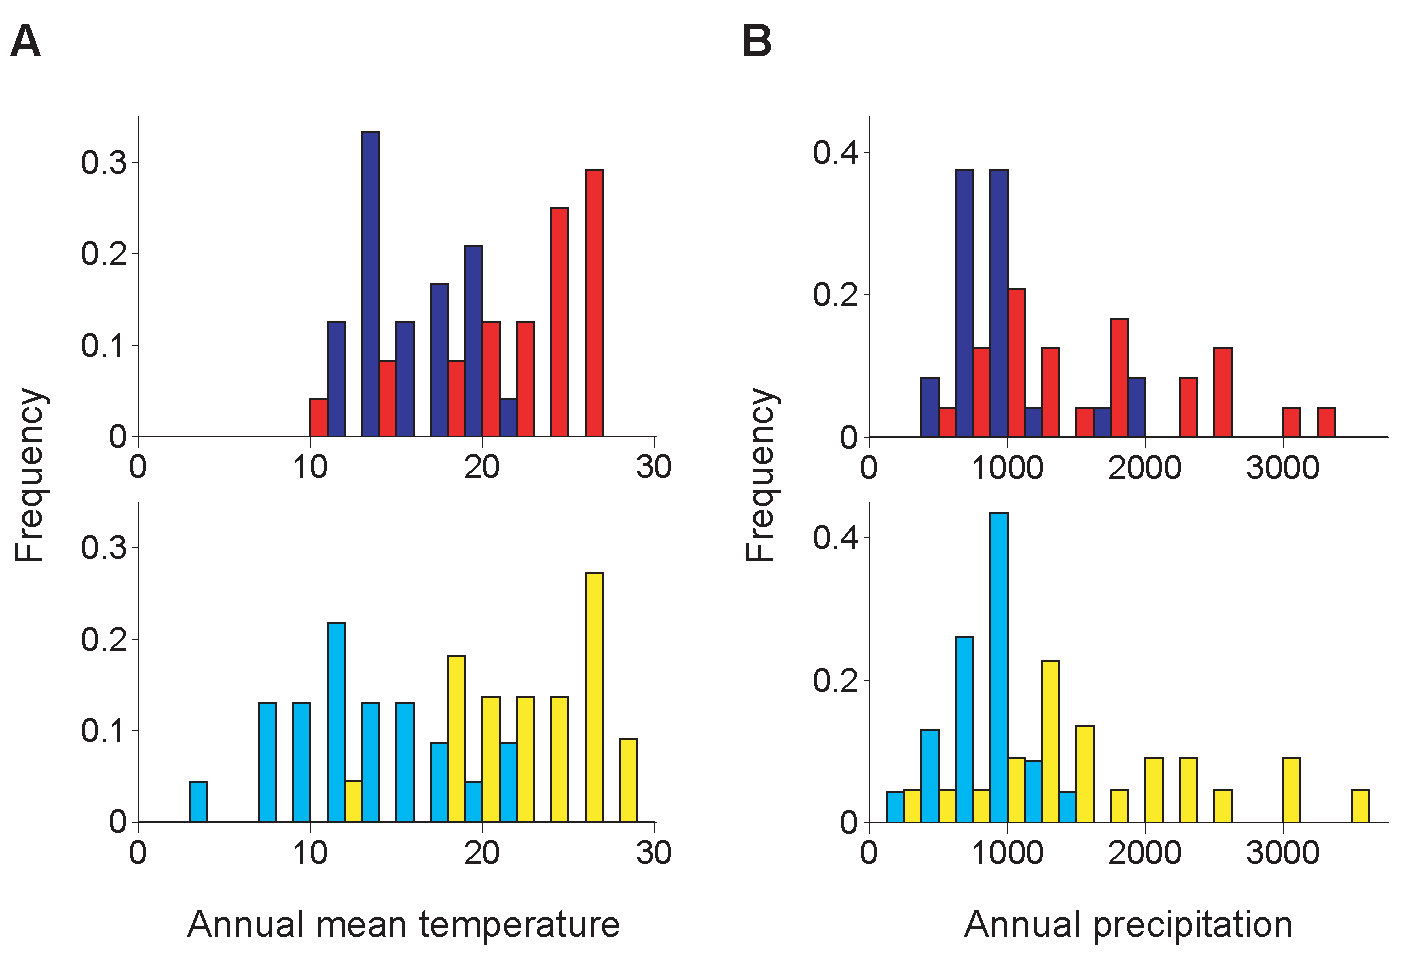
\includegraphics[width=0.6\columnwidth]{fig/bioclm.pdf}
    \caption{Correlation of allele frequencies between GBS (\emph{x}-axes) and MaizeSNP50 (\emph{y}-axes) data.  We used overlapped SNPs with $n\geq40$ for both data sets.  Correlation coefficient is 0.890 ($P<10^{-5}$ by permutation test with $10^5$ replications).}
    \label{colfreq}
  \end{center}
\end{figure}
%%%%%%%%%%%%%%%%%%%%%%%%%%%%%%%%%%%%%%%%%%%%%%%%%%%%%%%%%%%%

%%%%%%%%%%%%%%%%%%%%%%%%%%%%%%%%%%%%%%%%%%%%%%%%%%%%%%%%%%%%
\begin{figure}[t]
  \begin{center}
    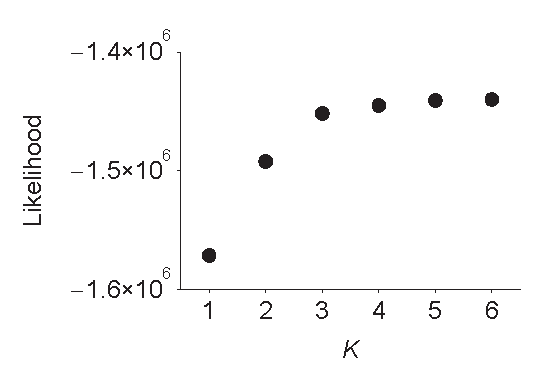
\includegraphics[width=0.4\columnwidth]{fig/kk.pdf}
    \caption{Likelihood of STRUCTURE analysis given $K$.  The \emph{x}-axes represents $K$ and the \emph{y}-axes represents likelihood.}
    \label{colfreq}
  \end{center}
\end{figure}
%%%%%%%%%%%%%%%%%%%%%%%%%%%%%%%%%%%%%%%%%%%%%%%%%%%%%%%%%%%%

%%%%%%%%%%%%%%%%%%%%%%%%%%%%%%%%%%%%%%%%%%%%%%%%%%%%%%%%%%%%
\begin{figure}[t]
  \begin{center}
    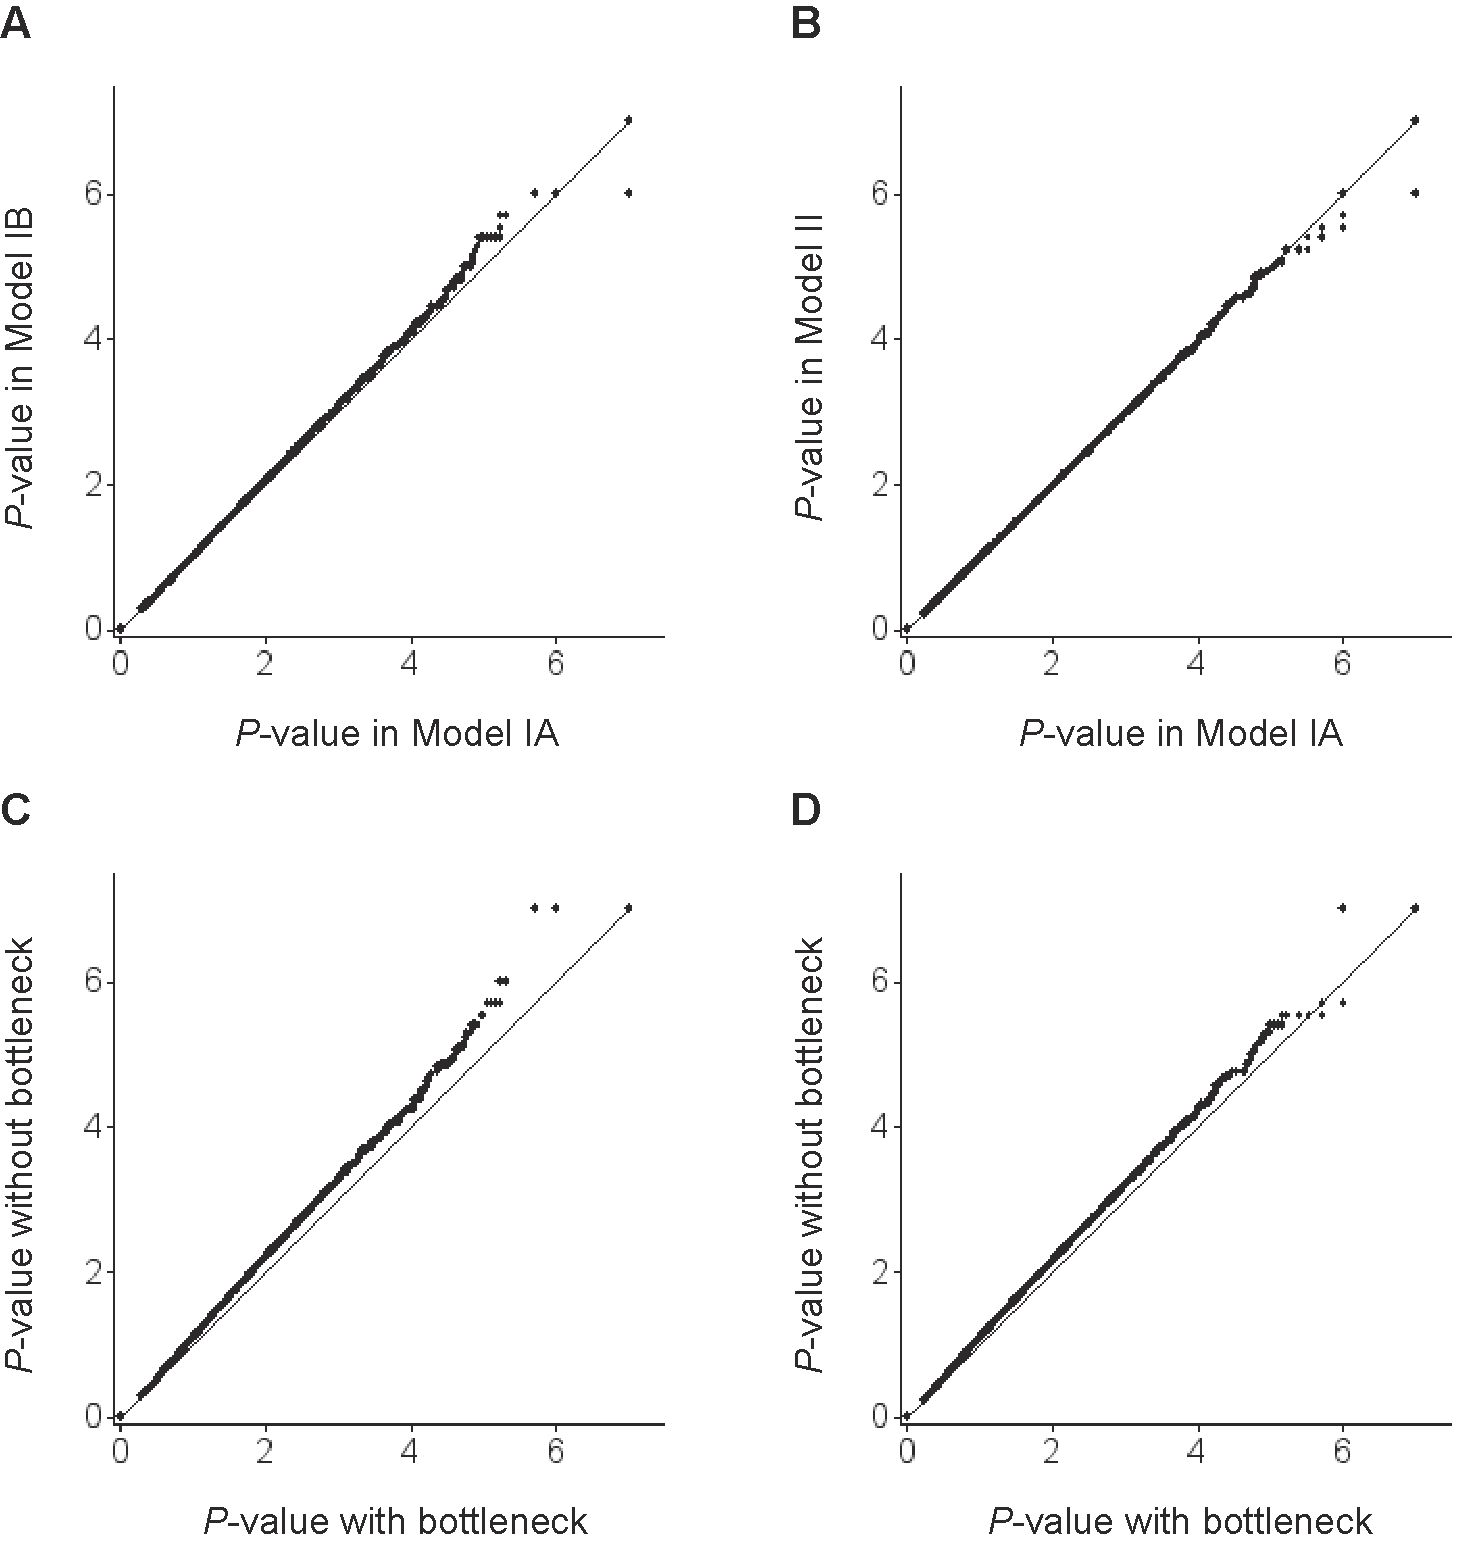
\includegraphics[width=0.6\columnwidth]{fig/bot2.pdf}
    \caption{Q-Q plot for $-$log$_{10}$-scaled \emph{P}-values of population differentiation between lowland and highland populations. (A) Model IA \emph{v.s.} Model IB in Mexico, (B) Model IA \emph{v.s.} Model II in S. America, (C) Model with \emph{v.s.} without bottleneck in Mexico and (D) Model with \emph{v.s.} without bottleneck in S. America.}
    \label{colfreq}
  \end{center}
\end{figure}
%%%%%%%%%%%%%%%%%%%%%%%%%%%%%%%%%%%%%%%%%%%%%%%%%%%%%%%%%%%%


%%%%%%%%%%%%%%%%%%%%%%%%%%%%%%%%%%%%%%%%%%%%%%%%%%%%%%%%%%%%
\begin{figure}[t]
  \begin{center}
    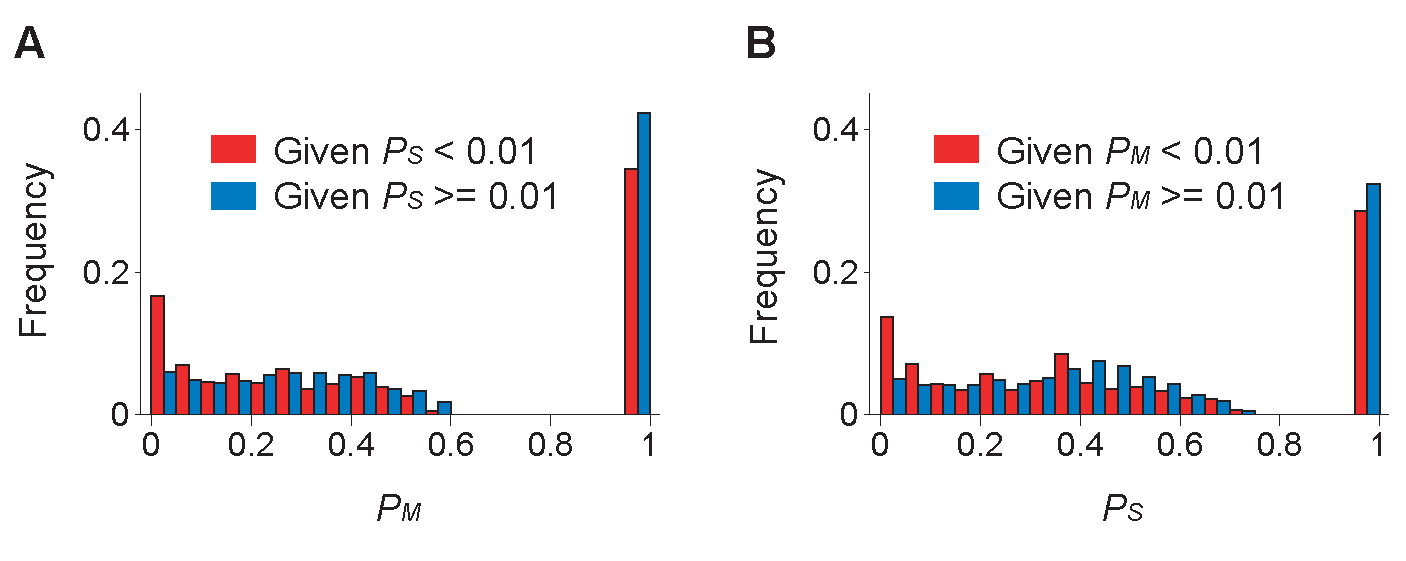
\includegraphics[width=0.8\columnwidth]{fig/pmps.pdf}
    \caption{(A) Frequency distribution of $P_M$ given $P_S<0.01$ and $P_S\geq0.01$.  (B) Frequency distribution of $P_S$ given $P_M<0.01$ and $P_M\geq0.01$.}
    \label{colfreq}
  \end{center}
\end{figure}
%%%%%%%%%%%%%%%%%%%%%%%%%%%%%%%%%%%%%%%%%%%%%%%%%%%%%%%%%%%%

%%%%%%%%%%%%%%%%%%%%%%%%%%%%%%%%%%%%%%%%%%%%%%%%%%%%%%%%%%%%
\begin{figure}[t]
  \begin{center}
    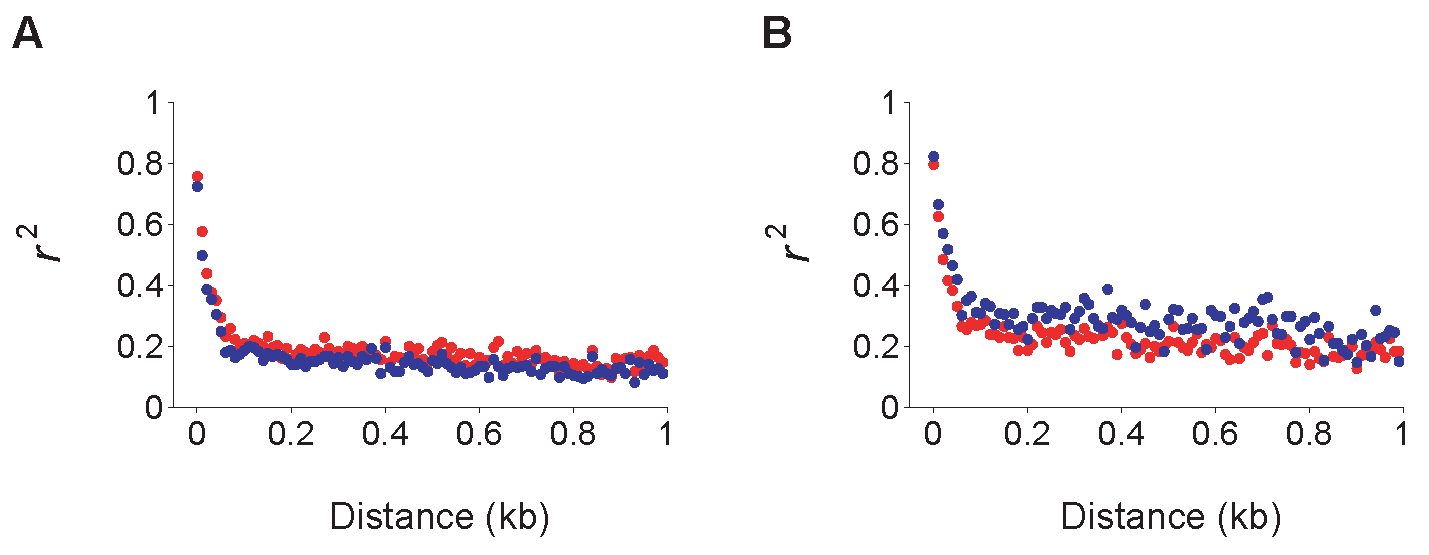
\includegraphics[width=0.7\columnwidth]{fig/LD.pdf}
    \caption{Pattern of decay of linkage equilibrium in Mexico (A) and South America (B).  Red and blue dots represent low- and highland population, respectively.  $r^2$ values were calculated as a statistics and averaged within 10-bp bins of distance between SNPs.  The \emph{x}- and \emph{y}-axes represent distance between SNPs (kb) and average $r^2$ values.}
    \label{colfreq}
  \end{center}
\end{figure}
%%%%%%%%%%%%%%%%%%%%%%%%%%%%%%%%%%%%%%%%%%%%%%%%%%%%%%%%%%%%


%%%%%%%%%%%%%%%%%%%%%%%%%%%%%%%%%%%%%%%%%%%%%%%%%%%%%%%%%%%%
\begin{figure}[t]
  \begin{center}
    \includegraphics[width=0.4\columnwidth]{fig/col.pdf}
    \caption{Correlation of allele frequencies between GBS (\emph{x}-axes) and MaizeSNP50 (\emph{y}-axes) data.  We used overlapped SNPs with $n\geq40$ for both data sets.  Correlation coefficient is 0.890 ($P<10^{-5}$ by permutation test with $10^5$ replications).}
    \label{colfreq}
  \end{center}
\end{figure}
%%%%%%%%%%%%%%%%%%%%%%%%%%%%%%%%%%%%%%%%%%%%%%%%%%%%%%%%%%%%





%%%%%%%%%%%%%%%%%%%%%%%%%%%%%%%%%%%%%%%%%%%%%%%%%%%%%%%%%%%%
%\begin{figure}[t]
%  \begin{center}
%    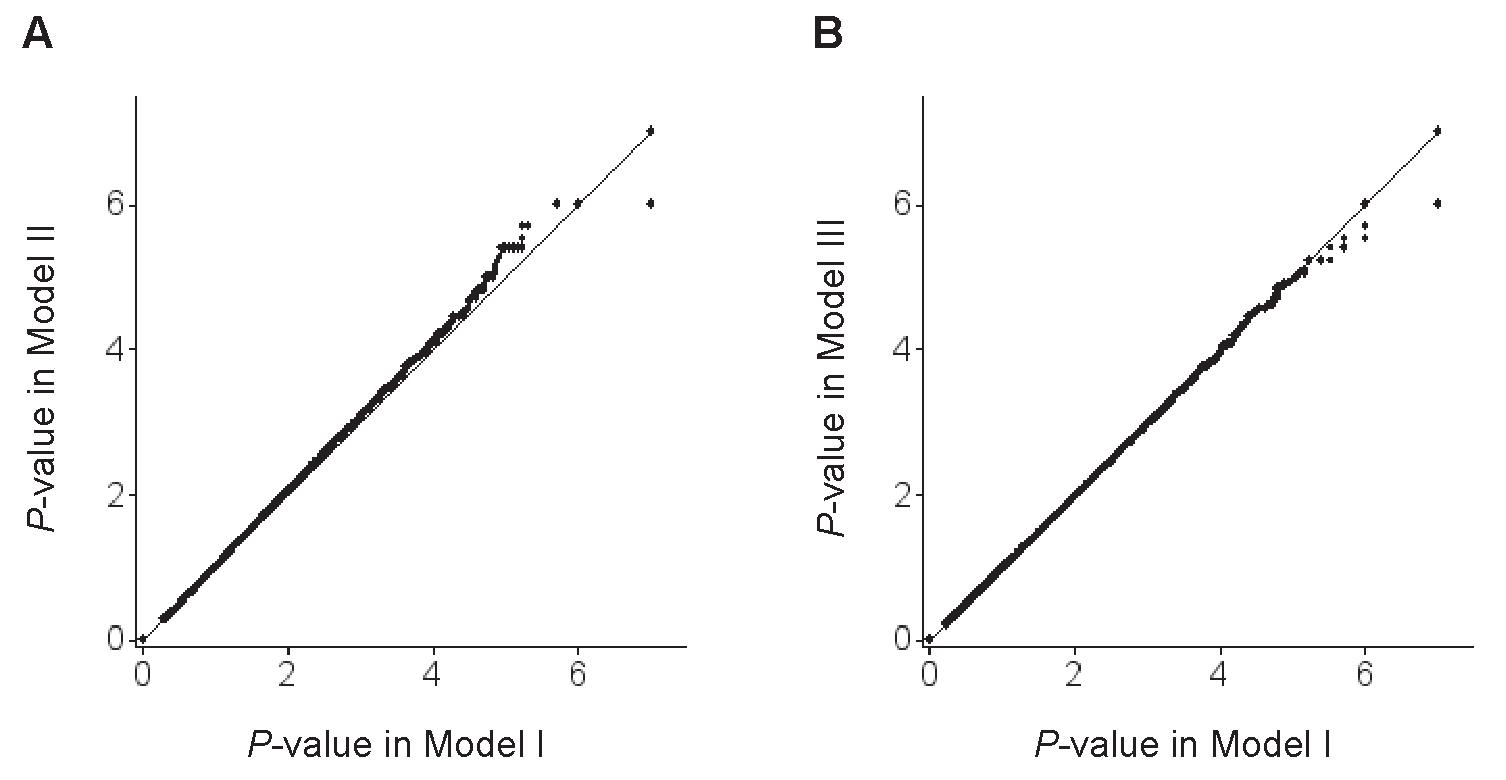
\includegraphics[width=0.6\columnwidth]{fig/GBSP.pdf}
%    \caption{Q-Q plot for $-$log$_{10}$-scaled \emph{P}-values of population differentiation between models in GBS data. The results of Mexico (A) and South America (B) are shown. The solid lines represent \emph{y}=\emph{x}.}
%    \label{colfreq}
%  \end{center}
%\end{figure}
%%%%%%%%%%%%%%%%%%%%%%%%%%%%%%%%%%%%%%%%%%%%%%%%%%%%%%%%%%%%



%%%%%%%%%%%%%%%%%%%%%%%%%%%%%%%%%%%%%%%%%%%%%%%%%%%%%%%%%%%%
%\begin{figure}[t]
%  \begin{center}
%    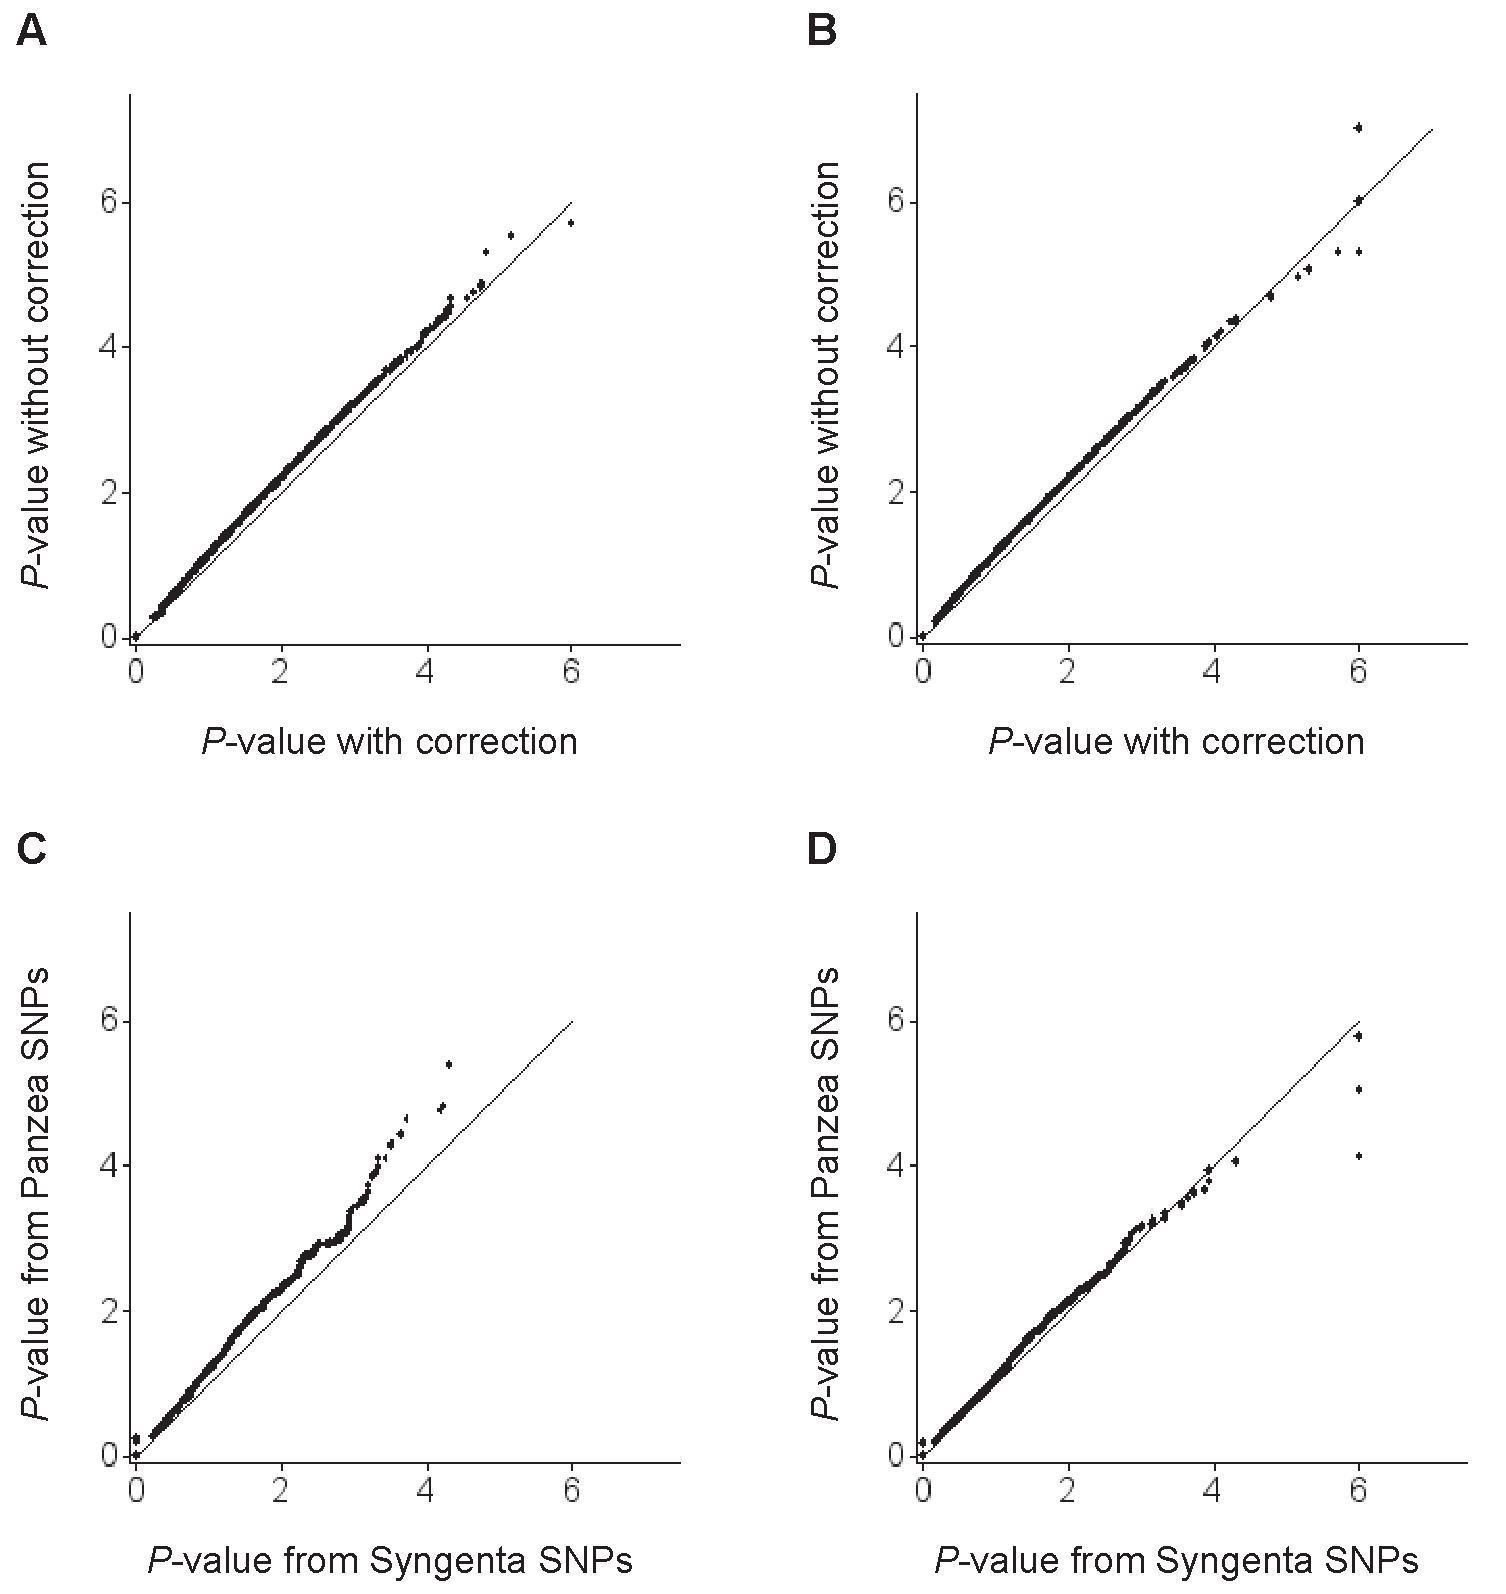
\includegraphics[width=0.6\columnwidth]{fig/MZ50P.pdf}
%    \caption{Q-Q plot for $-$log$_{10}$-scaled \emph{P}-values in MaizeSNP50 data.  (A, B) Q-Q plot of \emph{P}-values with and without correlation of ascertainment bias (on the \emph{x}- and \emph{y}-axes, respectively) in Mexico (A) and South America (B).   (C, D) Q-Q plot of \emph{P}-values from Syngenta SNPs on the \emph{x}-axes and from Panzea SNPs on the \emph{y}-axes in Mexico (C) and South America (D).  The solid lines represent \emph{y}=\emph{x}.}
%    \label{colfreq}
%  \end{center}
%\end{figure}
%%%%%%%%%%%%%%%%%%%%%%%%%%%%%%%%%%%%%%%%%%%%%%%%%%%%%%%%%%%%





\end{document}










